\documentclass[]{article}
\usepackage[utf8]{inputenc}
\usepackage{pdfpages}
\usepackage{amsmath}
\usepackage{amssymb}
\usepackage{graphicx}
\usepackage{geometry}
\usepackage{enumitem}
\usepackage{amsthm}
\usepackage{stmaryrd}
\usepackage{mathtools}
\usepackage{mathrsfs}
\usepackage{bbm}

\geometry{hmargin=2cm}

% Environnement type théorème
\newtheorem{mythm}{Théorème}
\newtheorem{myproposition}{Proposition}
\newtheorem{myproperty}{Propriété}
\newtheorem{mylemma}{Lemme}
\newtheorem{mycoro}{Corollaire}

% Environnement type texte
\theoremstyle{remark}
\newtheorem{mynot}{Notation}
\newtheorem{myrem}{Remarque}
\newtheorem{myexer}{Exercice}
\newtheorem{myproof}{Preuve}
\newtheorem{myexmpl}{Exemple}

% Environnement de définition
\theoremstyle{definition}
\newtheorem{mydef}{Définition}
\newtheorem{myquestion}{Question}

\setlist[itemize]{label=-}

% Carré de fin de preuve
\newcommand{\cqfd}{
	\hfill$\square$
}

% Définition de fonction
\newcommand{\func}[5]{
#1 ~ : ~ \left\{ \begin{array}{lcl}
	#2 & \longrightarrow & #3 \\
	#4 & \longmapsto & #5
\end{array}
\right.
}

\newcommand{\fun}[3]{
#1 ~ : ~ #2 \longrightarrow #3
}

\newcommand{\funcinline}[5]{
	#1 \, : \, #2 \longrightarrow #3, ~ #4 \longmapsto #5
}

\newcommand{\funcshort}[3]{
	#1 \, : \, #2 \longrightarrow #3
}

\newcommand{\anonfunc}[4]{
	\left\{ \begin{array}{lcl}
		#1 & \longrightarrow & #2 \\
		#3 & \longmapsto & #4
	\end{array}
	\right.
}

\newcommand{\vect}{\text{Vect}}

\newcommand{\card}{\text{Card }}

\newcommand{\DS}{\displaystyle}

\begin{document}
	\part{Analyse du signal}
	
	On munit à présent $L^2(\mathbb{R})$ du produit scalaire $\langle \cdot, \cdot \rangle$ défini par $$\langle f, g\rangle = \int_\mathbb{R} f(t) \overline{g(t)} dt$$
	
	[On considérera ici que $L^2(\mathbb{R})$ est restreint aux fonctions continues par morceaux ?]
	
	\section{Analyse multi-résolution}
	
	\subsection{Introduction}
	
	Nous allons enrichir la théorie des espaces de Hilbert d'une notion de "finesse"  particulièrement adaptée à l'objet central de ce rapport. En effet, dans le cadre de l'approximation d'un signal, que nous modélisons par une fonction $\mathbb{R}^n \rightarrow \mathbb{R}^m$, cette notion prend tout son sens comme le montre l'image ci-dessous.
	
	\begin{figure}[h]
		\centering
		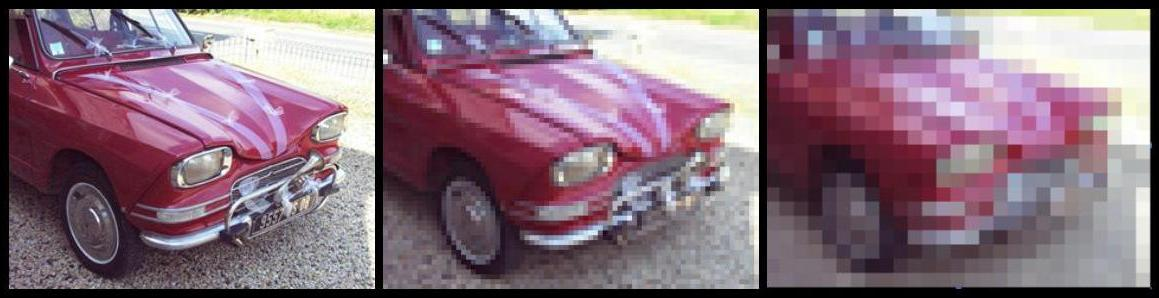
\includegraphics[width=350pt]{Resolution_wikipedia.jpg}
		\caption{Une image de voiture pour trois résolutions différentes}
	\end{figure}
	
	Les images peuvent être modélisées comme des fonctions de $\mathbb{R}^2$, pour les coordonnées spatiales, dans $\mathbb{R}$ (resp. $\mathbb{R}^3$) dans le cas d'une image en noir et blanc (resp. en couleur RVB). Dans le cas d'un signal sonore, sachant qu'un son est une onde, il peut être représenté par une fonction de $\mathbb{R}$, pour le temps, dans $\mathbb{R}$, pour l'amplitude de d'oscillation.
	
	Avant de définir l'analyse multi-résolution, explorons plus profondément cette notion de "finesse".
	
	\subsubsection*{Quelle finesse !}
	
	Nous allons prendre pour exemple les signaux unidimensionnels (tels les sons). Soit $\funcshort{f}{[0, 1[}{\mathbb{R}}$ une fonction continue, nous allons l'approximer par des fonctions constantes par morceaux (dites étagées), dont les morceaux sont de plus en plus petits.
	
	\begin{figure}[h]
		\centering
		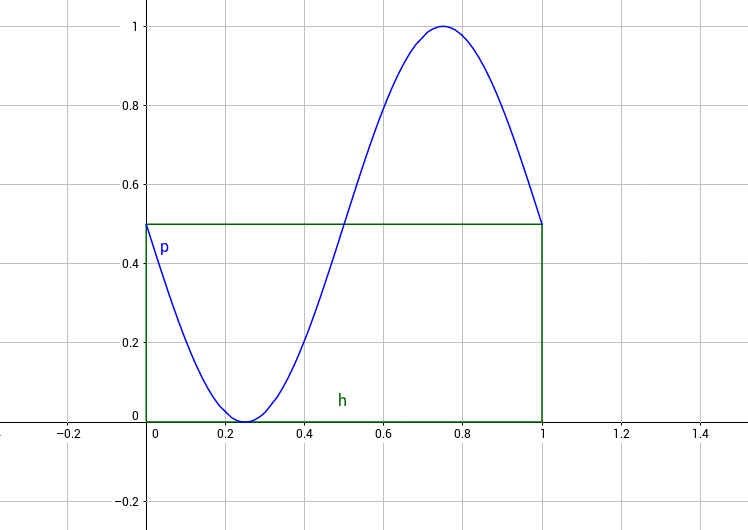
\includegraphics[width=150pt]{sin_1.png}
		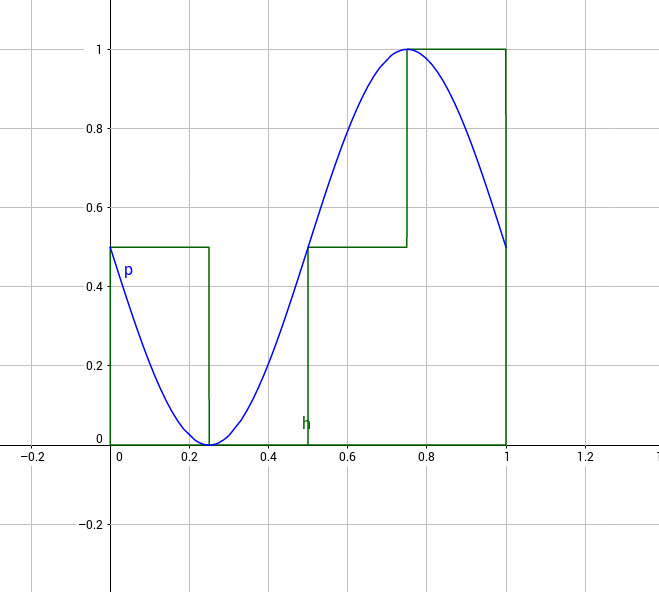
\includegraphics[width=150pt]{sin_2.png}
		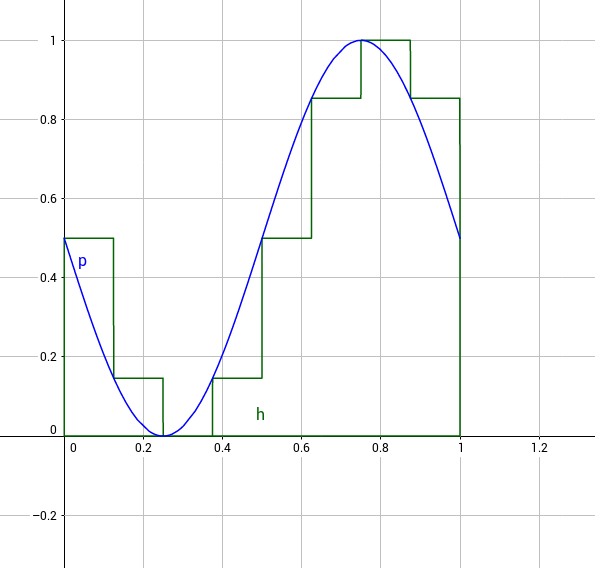
\includegraphics[width=150pt]{sin_4.png}
		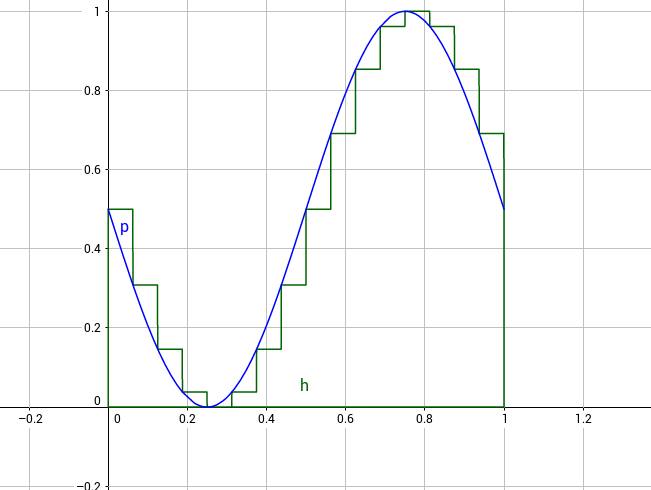
\includegraphics[width=150pt]{sin_8.png}
		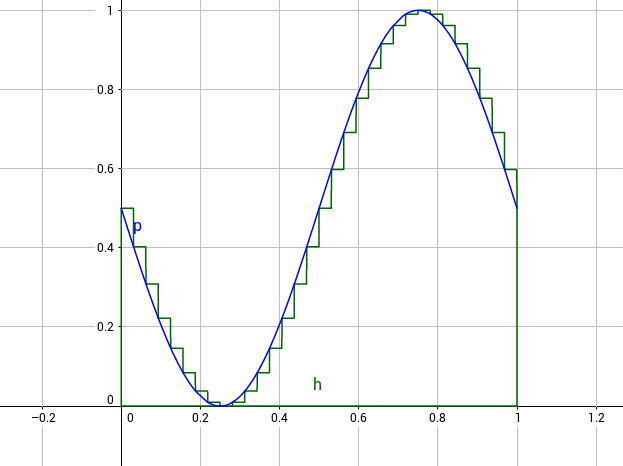
\includegraphics[width=150pt]{sin_16.png}
		\caption{$f$ approximée par des fonctions dont les morceaux sont de tailles 1, 1/2, 1/4, 1/8 et 1/16}
	\end{figure}
	
	\newpage
	
	Sur la figure on approxime $f$ par des fonctions $f_n$ étagées dont les morceaux sont de tailles $2^{-n}$, on peut voir chaque $f_n$ comme une combinaison linéaire de fonctions caractéristiques de la forme suivante $$f_n = \sum_{k = 0}^{2^n} a_{n, k} \mathbbm{1}_{[k 2^{-n}, (k+1)2^{-n}[}$$
	
	La première remarque que l'ont peut faire est que chaque $\mathbbm{1}_{[k 2^{-n}, (k+1)2^{-n}[}$ est le translaté de $\mathbbm{1}_{[0, 2^{-n}[}$, que l'on notera $I_n$. On réécrit alors $$f_n(x) = \sum_{k = 0}^{2^n} a_{n, k} I_n\left(x - k 2^{-n}\right)$$
	
	La seconde est que $I_n$ est une contraction de $I_1$ que l'on notera $I$. On en tire notre dernière réécriture :
	
	$$f_n(x) = \sum_{k = 0}^{2^n} a_{n, k} I \left(\frac{x - k 2^{-n}}{2^{-n}}\right) = \sum_{k = 0}^{2^n} a_{n, k} I \left(2^n x - k\right)$$
	
	Ainsi si on fixe $I = \mathbbm{1}_{[0, 1[}$ comme fonction de référence dans notre décomposition, la suite de fonctions $(f_n)_n$ est entièrement déterminée par les coefficients $(a_{n, k})_{n, k}$
	
	\subsection{L'analyse multi-résolution}
	
	Dans l'exemple introductif, pour tout $n$ on a pu voir que $f_n$ était une combinaison linéaire du translaté d'une fonction $I_n$, $f_n$ appartenait alors à l'espace vectoriel engendré par les translations de $I_n$. De plus, chaque $I_n$ était la contraction de la fonction $I$ donnée par $I_n(t) = I\left(t 2^n\right)$. Il s'agissait d'un exemple d'analyse multi-résolution dont voici la définition :
	
	\begin{mydef}
		Une \textit{analyse multi-résolution} de l'espace $L^2(\mathbb{R})$ des fonctions de carré Lebesgue-intégrables est une suite $V = \{V_n\}_{n \in \mathbb{Z}} \subset L^2(\mathbb{R})$ de sous-espaces fermés de $L^2(\mathbb{R})$ satisfaisant aux conditions suivantes :

		\begin{enumerate}
			\item $\forall n \in \mathbb{Z}, ~ V_{n} \subset V_{n+1}$ \textit{(croissance)}
			\item $\forall n \in \mathbb{Z}, \forall f \in L^2(\mathbb{R}), ~ f \in V_n \Longleftrightarrow t \mapsto f \left(2 t\right) \in V_{n+1}$ \textit{(stabilité par translation entière)}
			\item $\forall n \in \mathbb{Z}, \forall f \in L^2(\mathbb{R}), ~ t \mapsto f \left(t + 2^n\right) \in V_n \Longleftrightarrow f \in V_n$ \textit{(auto-similarité)}
			\item $\DS \overline{\bigcup V} = L^2(\mathbb{R})$ \textit{(densité)}
			\item $\DS \bigcap V = \{0\}$
		\end{enumerate}
	\end{mydef}
	
	On peut généraliser par récurrence la propriété 3 de la façon suivante :
		
	$$\forall n \in \mathbb{Z}, \forall f \in L^2(\mathbb{R}), ~ f \in V_0 \Longleftrightarrow t \mapsto f \left(2^n t\right) \in V_{n}$$

	Ce qui met en évidence que plus $n$ est grand, plus l'espace $V_n$ contient des fonctions fines (la fonction est contractée horizontalement). La propriété 4 peut elle aussi être généralisée :
		
	$$\forall n \in \mathbb{Z}, \forall k \in \mathbb{Z}, \forall f \in L^2(\mathbb{R}), ~ f \in V_n \Longleftrightarrow t \mapsto f \left(t -k 2^n\right) \in V_{n}$$
	
	En combinant ces deux conséquences, on sait alors qu'une fonction $f$ appartient à $V_n$ si et seulement s'il existe $\varphi \in V_0$, $k \in \mathbb{Z}$ tels que $f(t) = \varphi (t 2^n - k)$.
	
	\begin{mydef}
		S'il existe une fonction normée dont l'ensemble de ses translations forme une base orthonormée de $V_0$, on l'appelle \textit{fonction d'échelle}. Ainsi pour tout $n$ l'espace $V_n$ est l'ensemble de combinaisons linéaires de dilatations et translations de cette fonction.
	\end{mydef}
	Nous nous retrouvons pour tout $n$ avec un espaces de Hilbert $V_n$ de base orthonormée $\{t \to 2^{-n/2} \varphi(2^n t - k) ~ | ~ k \in \mathbb{Z}\}$ (le facteur $2^{-n/2}$ servant à normaliser la fonction).
	
%	\begin{myexmpl}
%		On reprend l'exemple précédent, avec $\varphi = \mathbbm{1}_{[0, 1[}$. On a alors pour tout $n, k \in \mathbb{Z}$ $$\varphi_{n, k} = 2^{n/2} \mathbbm{1}_{[k 2^{-n}, (k+1) 2^{-n}[}$$
%		
%		Pour tout entier $n$, la famille $\left(\varphi_{n, k}\right)_{k \in \mathbb{Z}}$ est effectivement une famille orthonormée : 
%		\begin{align*}
%			\langle \varphi_{n, k}, \varphi_{n, k'} \rangle &= \int_{\mathbb{R}} \varphi_{n, k} \varphi_{n', k'} d \lambda \\
%			&= \int_{\mathbb{R}} 2^{-n}  \mathbbm{1}_{[k 2^{-n}, (k+1) 2^{-n}[} \mathbbm{1}_{[k' 2^{-n}, (k'+1) 2^{-n}[} d \lambda \\
%			&= 2^{n}  \int_{\mathbb{R}} \mathbbm{1}_{[k 2^{-n}, (k+1) 2^{-n}[ \cap [k' 2^{-n}, (k'+1) 2^{-n}[} d\lambda \\
%			&= 2^{n} \lambda\left([k 2^{-n}, (k+1) 2^{-n}[ \cap [k' 2^{-n}, (k'+1) 2^{n}[\right)
%		\end{align*}
%		
%		On voit bien que les ensembles $[k 2^{-n}, (k+1) 2^{-n}[$ sont disjoints, donc la mesure de l'intersection considérée est soit nulle (si $k \neq k'$), soit égale à $\lambda([k 2^{-n}, (k+1) 2^{-n}[) = 2^{-n}$ (si $k = k'$).
%		
%		On retrouve bien $$\langle \varphi_{n, k}, \varphi_{n, k'} \rangle = \delta_{k, k'}$$
%		
%		On peut de plus approximer toute fonction de $L^2(\mathbb{R})$ aussi finement que souhaité par une fonction de $\DS \bigcup_{n \in \mathbb{Z}} V_n$.
%		
%		* Mq $V_n$ fermé
%		
%		* Mq toute fonction peut être approximé avec une finesse arbitraire par un élément de $\bigcup V$
%	\end{myexmpl}
		
	\subsection{Espace des détails}
	
	Lorsque l'on passe d'un espace $V_{n+1}$ à $V_{n}$, on perd en finesse. On regroupe l'espace qui engendre les détails perdus dans l'espace de détails :
	
	\begin{mydef}
		Pour tout $n$ on définit \textit{l'espace de détails} $W_{n}$ comme le complémentaire orthogonal de $V_{n}$ dans $V_{n+1}$ $$V_{n+1} = W_n \stackrel{\perp}{\oplus} V_n$$
	\end{mydef}
	
	\begin{myrem}
		Toute fonction $f \in \bigcup V$ se décompose de manière unique en une somme de fonctions orthogonales $f = f_1 + f_2$, où $f_1 \in V_{n}$ et $f_2 \in W_n$ pour un certain $n$.
		
		En effet, $f \in \bigcup V$ donc il existe $n$ tel que $f \in V_n$. Il s'agit donc d'une combinaison linéaire de translations et contractions d'un facteur au plus $2^{-n}$ de $\varphi$. Il existe d'uniques éléments $f_1 \in V_{n-1}$ et $f_2 \in W_{n-1}$ tels que $f = f_1 + f_2$ et $f_2 ~ \bot ~ f_2$.
		
		Le fait que $f_1$ et $f_2$ soit orthogonaux signifie que $f_1 \overline{f_2}$ est d'intégrale nulle.
		
		$f_2$ peut être vu comme le détail perdu en passant de l'échelle $V_n$ à l'échelle $V_{n-1}$.
	\end{myrem}
	
	Les $(W_n)_n$ ne forment plus une famille monotone, mais leur somme recouvre tout les $V_n$. En d'autre termes, on peut à présent approximer toute fonction de $L^2(\mathbb{R})$ par une combinaison linéaire d'éléments de $\DS \bigoplus_{n \in \mathbb{Z}} W_n$.
	
	\begin{myproof}
		Soit $n_0 \in \mathbb{Z}$, on a par définition des $(W_{n})_n$
		
		\begin{align*}
			V_{n_0+1} &= V_{n_0} \oplus W_{n_0} \\
			&= V_{n_0 - 1} \oplus \left(W_{n_0 - 1} \oplus W_{n_0} \right) \\
			& \cdots \\
			&= V_{n_0 - N} \oplus \left(\bigoplus_{n = n_0 - N}^{n_0} W_n \right) \\
			&= \cdots \\
			&= \lim\limits_{n \to -\infty} V_n \oplus \left(\bigoplus_{n = - \infty}^{n_0} W_n \right) \\
			&= \bigcap V \oplus \left(\bigoplus_{n = - \infty}^{n_0} W_n \right) \\
			&= \{0\} \oplus \left(\bigoplus_{n = - \infty}^{n_0} W_n \right) \\
			&= \bigoplus_{n = - \infty}^{n_0} W_n
		\end{align*}
		
		On en déduit ainsi $\DS \bigcup V = \bigoplus_{n \in \mathbb{Z}} W_n$ en faisant tendre $n_0$ vers $\infty$ (ou plutôt en faisant l'union à gauche et à droite pour tout $n_0 \in \mathbb{Z}$).
		
		\cqfd
	\end{myproof}
	
	Comme on l'a dit, les $(W_n)_n$ ne forment pas une suite d'espaces emboîtés ; ils sont même orthogonaux deux à deux. Cependant, ils vérifient encore les conditions d'auto-similarité et de stabilité par translation.

	\begin{mydef}
		Si on peut encore trouver une fonction normée $\psi$ engendrant $W_0$ par translation et de moyenne nulle (d'intégrale nulle), une telle fonction est appelée \textit{ondelette}.
	\end{mydef}
	
	On définit encore une fois la famille $(\psi_{n, k})_{n, k}$ par $\psi_{n, k}(t) = 2^{-n/2} \psi(2^{n} t - k)$, et cette fois ci ... cette famille est une base orthonormée de $\DS \bigoplus_{n \in \mathbb{Z}} W_n$ !
	
	Le fait que la famille soit normée est évident, le fait qu'elle soit orthogonale découle de l'orthogonalité des $W_n$.
	
\end{document}